\documentclass[12pt, a4paper]{article}
\usepackage[margin=1in] {geometry}
\usepackage[english]{babel}
\usepackage[T1]{fontenc}
\usepackage[utf8]{inputenc}
\usepackage{setspace}
\usepackage{graphicx}
\usepackage{float}
\usepackage{amsmath}
\usepackage{arydshln}
\usepackage{enumitem}
\usepackage[backend=biber,style=numeric,sorting=none]{biblatex}
\addbibresource{biblio.bib}
\usepackage{algorithm}
\usepackage{algpseudocode}



\usepackage{url}

\begin{document}

\thispagestyle{empty}
\begin{center}
    \vspace*{3cm}
    {\large Project of: Marco Colangelo (Student ID: 67045A)}\\[0.3cm]
    {\large Algorithms for Massive Datasets, Academic Year 2024/25}\\[0.3cm]
    {\large Master's Degree in Computer Science, University of Milan}\\[1.2cm]

    {\LARGE\bfseries
    Finding Similar Amazon Books Reviews\\
    using LSH, MinHashing and Jaccard Similarity}\\[1.2cm]

    {\large September 4, 2025}
\end{center}

\setcounter{page}{1}

\section{Introduction}
This report contains an overall on the work carried out for the final project of the course of Algorithms for Massive Datasets. The professor in charge of the course is Professor Dario Malchiodi and the course was taught at the University of Milan in the second semester of the 2024/25 academic year.

Among the various assignments for the project, all consistent with the topics presented in the course, this work focused on the problem of \textbf{finding similar items}. More specifically, the work focused on the implementation of a specific procedure presented in the course for finding similar items, which combines MinHashing and Locality-Sensitive Hashing (LSH) techniques to find similar items using Jaccard Similarity. These techniques will be examined in detail later in this report, particularly their theoretical foundations and how they have been implemented and parameterized.

For the project, the dataset used is Amazon Books Reviews, made available on Kaggle and containing information about various books and user reviews associated with those books. The version used for this project is the version 1, dated 14 September 2022, and the dataset is not pre-loaded but downloaded at runtime. The project focused on the task of finding similar reviews, using the full text of the reviews.

This project was built on Google Colab and is intended to run on a distributed computing environment. For this purpose, the PySpark library, which provides a Spark API for Python, was used. 

\section{The Amazon Books Reviews dataset}

The Amazon Books Reviews dataset, in the version used (version 1 of 2022), has a total size of approximately 3 gigabytes and consists of two tables:
\begin{itemize}
    \item \texttt{books\_rating}: has a total size of approximately 2.8 gigabytes 
    and contains 3 million reviews. The table has several columns: however, both 
    for the purposes of the work performed and to reduce the data loaded into memory, 
    the only columns retained were:
    \begin{itemize}
        \item \texttt{ID}: Unique ID for a book
        \item \texttt{User\_id}: The ID of the user who wrote the review
        \item \texttt{Title}: Title of the book
        \item \texttt{Review/text}: Contains the entire text of the review
    \end{itemize}
    For this dataset, the primary key (i.e. what characterizes a review) is made up of the pair of values \texttt{(ID, User\_id)}: this is the reason those columns were necessary. 
    \item \texttt{books\_data}: has a size of approximately 180 megabytes and 
    contains information for approximately 200000 books. 
    This table will not be considered, as the work performed focused on book reviews.
\end{itemize}
This dataset is downloaded at runtime and, as will be shown later, will be sampled randomly to ensure reasonably low execution times and memory requirements.


\section{Manipulation of the dataset}
The following section will explain how the dataset was manipulated for the purposes of the work performed, both in terms of subsampling and preprocessing applied.
\subsection{Dataset subsampling}
As shown previously, the \texttt{books\_rating} dataset used is large, which would significantly increase execution time on Google Colab. For this reason, the \texttt{books\_rating} dataset was sampled, randomly selecting 30000 elements.
\subsection{Dataset preprocessing}
First, only the \texttt{ID, Title, User\_id} and \texttt{review/text} columns were selected from the sample. The sample was then filtered to remove all rows with empty or null \texttt{review/text} columns, thus eliminating reviews of this type. The resulting sample has the following structure:
\begin{figure}[H]
    \centering
    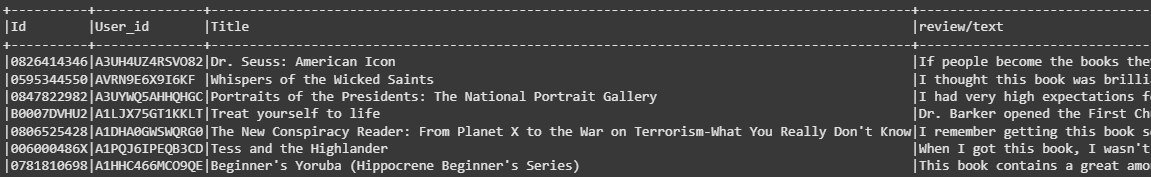
\includegraphics[width=\linewidth]{Screenshot 2025-09-04 103020.png}
    \caption{Structure of the sample used}
    \label{fig:placeholder}
\end{figure}
However, it should be noted that no row in the sample ever contained an empty or null review, but the filter was still applied to provide for the possibility of handling such cases.

The second preprocessing step applied was some kind of normalization of the \texttt{review/text} column for all rows in the sample. This normalization involved three steps:
\begin{enumerate}
    \item Converting the \textbf{entire text to lowercase}, so that a lowercase letter and an uppercase letter are not considered different (for example, "House" and "house" are the same word, but they do not have the same letters).
    \item \textbf{Removing punctuation marks and non-alphanumeric characters} as these would generate inconsistent shingles. With regard to \textbf{spaces}, it was decided to leave at least one space between words (if these are present, of course) and, when punctuation marks and non-alphanumeric characters were removed, these have been replaced with a single space. 
    \item \textbf{Removing all stop words} from the text, such as the, an, and, or and so on. The reason why they were removed is because they are rather frequent words in sentences and therefore do not provide a particularly informative contribution.
\end{enumerate}
After this preprocessing, a \texttt{review/text} occurrence went from this
\begin{figure}[H]
    \centering
    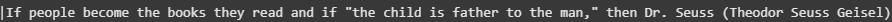
\includegraphics[width=\linewidth]{Screenshot 2025-09-04 103608.png}
    \caption{review/text before normalization}
    \label{fig:placeholder}
\end{figure}
to this
\begin{figure}[H]
    \centering
    
\includegraphics[width=\linewidth]{Screenshot 2025-09-04 103734.png}
    \caption{review/text after normalization}
    \label{fig:placeholder}
\end{figure}

\section{Jaccard similarity, MinHashing and LSH to find similar items}
\subsection{Jaccard similarity}
The course presented the problem of finding similar elements considering textual documents as well as the same problem but on non-textual documents. One metric used to determine how much two textual documents are similar is Jaccard similarity, defined as
\begin{equation}
J(A,B) = \frac{|A \cap B |}{|A \cup B|} \in [0,1]
\end{equation}

where A and B are the two textual documents. The closer it is to 1, the more similar the documents are.

\subsection{Shingling of text for Jaccard similarity}
A preprocessing technique for applying Jaccard similarity is \textbf{shingling the text content}: a shingle is a k-gram, a set of k atomic information, such as the individual characters that make up a word or sentence. The choice of the k parameter is very important, because if it is chosen too low, for example, it would cause many documents to share the same k-shingles and therefore appear similar, even if they actually are not. A general rule is the following:
\begin{quote}
    \textit{k should be chosen large enough so that the probability of any shingle appearing in a given document is low.}
\end{quote}
For the project, the \textbf{chosen value for k was 5}. This is because the length of the review texts in the dataset varies greatly, with both fairly short reviews and much longer ones. Choosing an ideal k parameter for very long reviews (around 8-9) would have penalized the shorter ones. For this reason, k = 5 was chosen as the value for the shingle length, as it represents a good compromise between shingle specificity and the quantity of shingles generated even for the shortest reviews.

Let's look at an example of transforming the text of a review into 5-character shingles. Returning to the previous example shown in Figures 2 and 3, some of the generated shingles would be as follows:
\begin{figure}[H]
    \centering
    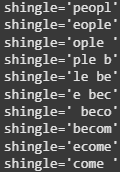
\includegraphics[width=0.25\textwidth]{Screenshot 2025-09-04 103955.png}
    \label{fig:placeholder}
\end{figure}

After the generation of the shingles, the next step is to create an encode for them. A simple approach is using hash functions. For the work done, an hash function 
\begin{equation}
    h: \{ \text{shingle}\} \to \{ 0\ldots2^{64} \}
\end{equation}
has been defined, specifically using the FNV-1a (Fowler-Noll-Vo version 1a) hash function \cite{wikipedia-fnv}. This hash function takes as input a shingle and produces as output an integer in the range between 0 and $2^{64}-1$, according to the following pseudocode:
\begin{center}
\begin{algorithm}[H]
\caption{Algoritmo FNV-1a}
\begin{algorithmic}[1]
\State $hash \gets FNV\_offset\_basis$
\ForAll{$byte\_of\_data$}
    \State $hash \gets hash \oplus byte\_of\_data$
    \State $hash \gets hash \times FNV\_prime$
\EndFor
\State \Return $hash$
\end{algorithmic}
\end{algorithm}
\end{center}

The following figure
\begin{figure}[H]
    \centering
    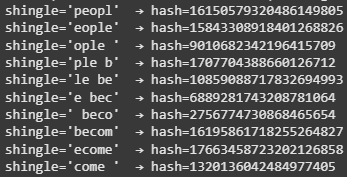
\includegraphics[width=0.5\textwidth]{Screenshot 2025-09-04 104157.png}
    \label{fig:placeholder}
\end{figure}
shows an example of this hash function applied to some of the shingles generated in the previous step.

In the lecterature, to visualize the relation between shingles a characteristic matrix (let's call it CM) can be constructed. This is a $s \times n$ matrix where s is the number of possible shingles and n is the number of documents and is defined as:
\begin{equation}
    CM_{ij} = 
    \begin{cases}
    1 \ \ \  \text{ if shingle i is contained in document j} \\ 
    0 \ \ \ \text{ otherwhise}
    \end{cases}
\end{equation}
There is a problem: this matrix is huge and sparse so we have to compress it, if we want to calculate it. This is where MinHashing comes in handy. 
\subsection{MinHashing}
MinHashing is a data compression method that allows us to efficiently estimate Jaccard similarity between sets without having to work directly with the full sets or characteristic matrix. The steps it requires are the following: 
\begin{enumerate}
    \item A row permutation of the characteristic matrix choosing a certain hash function.
    \item $\forall$ documents, scan its document column in the matrix until the fist 1, and return the corresponding shingle row.
    \item Construction of the Signature Matrix (let's call it SM), which columns are intended as signatures and define a document. A signature is an array of values, each corresponding to the output of an hash function applied after a permutation of the rows. It's a compact representation of the characteristic matrix.
\end{enumerate}
In the work done, \textbf{the number H of independent hash functions choosen was 128}, which has been resulted as a good compromise between the accuracy of the Jaccard similarity and the computational cost required. Every hash function is in the form of
\begin{equation}
    h_i(x) = (a_i\cdot x + b_i) \text{ mod p} 
\end{equation}
where $a_i$ and $b_i$ are casual values with fixed seed for reproducibility, p is a large prime number and x is the encode of the shingle. The reasons behind the choise of this hash function are several: first of all, is very simple to calculate, which is ideal for large datasets. Second, picked a and b randomly, the probability that two distinct values $x_1$ and $x_2$ collides is limited. Finally, for MinHashing a lot of independent hash functions are required and varying a and b makes sure that each hash function behave like a different permutation in the space of the shingles. 

%Let's see these hash function in action in the work done:

Using these hash functions allows us to exploit a very important theorem that further reduces computational cost. The hash functions used are random functions: that is, each time the characteristic matrix is observed, a permutation is randomly (and uniformly) chosen and the MinHashing is calculated. We define as E the event $H(D_1) = H(D_2)$ where $D_1$ and $D_2$ are two documents: this means that in the permuted matrix, for a given hash function h, the two documents $D_1$ and $D_2$ will have the same value k.

It can be shown that
\begin{equation}
    P(E) = J(D_1, D_2)
\end{equation}
that is, the number of favorable cases in which $H(D_1) = H(D_2)$, among all possible ones, is exactly the Jaccard similarity of the two documents.

This theorem allows us to estimate the Jaccard similarity between two documents $D_1$ and $D_2$ by simply calculating the ratio between the rows of the matrix where $D_1 = D_2$ and all the rows of the matrix. Formally
\begin{equation}
    \hat{J}(A,B) = \frac{\text{Lines where } D_1 = D_2}{\text{All lines}}
\end{equation}
This is how Jaccard similarity has been calculated to find similar reviews.

We see the satisfaction of this theorem in the work performed: 3000 elements were randomly selected from the sample, and for each pair in this sample, the exact Jaccard similarity was calculated on the set of their shingles and the estimated Jaccard similarity using the signatures produced by MinHashing. Subsequently, the RMSE was calculated to measure the average error between the estimated and exact Jaccard similarity, and a correlation graph was constructed where each point corresponds to a pair of documents, the x-axis corresponding to the exact Jaccard similarity, and the y-axis corresponding to the estimated Jaccard similarity. The RMSE obtained was approximately 0.0114, a value close to 0, indicating a low error in the calculated estimate. Let's now analyze the constructed graph:
\begin{figure}[H]
    \centering
    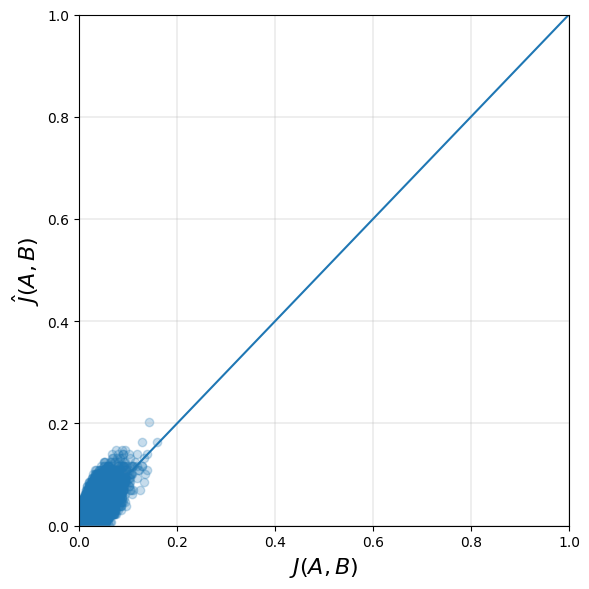
\includegraphics[width=0.5\textwidth]{Screenshot_2.png}
    \label{fig:placeholder}
\end{figure}
It can be seen how the values are distributed along the bisector, indicating that the estimate is very close to the true value. The reason why most of the points are located in the lower left indicates that the Jaccard similarity values are not particularly high, but they are compatible with the sample size used.

Speaking about the Signature Matrix, in the work done this data structure was implemented using Spark's Resilient Distributed Datasets (RDDs). This was because the signature matrix would have been large anyway, and given the desire to leverage a distributed computing environment, this was the preferred approach. Specifically, here's what was done:
\begin{enumerate}
    \item For each document, a MinHash of length H = 128 was calculated using the previously specified hash function.
    \item These MinHashes were saved as an array of length H and associated with the encoded document ID. This resulted in an RDD of pairs of the form \texttt{(document$\_$ID, signature$\_$vector)}, each of which can be thought of as a sparse column of the signature matrix. This is then used in LSH for the banding phase and for matching signatures to estimate Jaccard similarity.
\end{enumerate}

There is a practical problem: computing all the possible permutations of a set is time-consuming, but we can use hash functions to simulate the effect of a random permutation. Time complexity, however, remains prohibitive: having 1 milion documents, each of which consists of 250 4 bytes words, we would have a total of 1 gigabyte. If we suppose that each document is checked in 1 $\mu s
$, this would require about 5-6 days of total computational time, which is not the ideal for large datasets. This is where LSH comes in handy because it reduces the number of potential pairs of similar reviews to be considered. 
\subsection{Locality-Sensitive Hashing (LSH)}
Locality-sensitive hashing is a technique that significantly reduces time complexity by drastically reducing the number of document pairs to compare, selecting only a subset of candidates that are highly likely to be similar, or, in other words, with a Jaccard similarity above a certain threshold. Candidate pairs are those that are hashed to the same bucket, and Jaccard similarity is calculated only for these.

The idea is to divide the signature matrix into b bands of r rows each, and each band is associated with a hash function that takes a vector of r integers and hashes them to buckets. This means that if two documents are similar and should be considered potential candidates, then at least one of their bands must be identical. It can be shown that, by defining the event E = "The two documents have the same projection (or sub-signature) in at least one band," then
\begin{equation}
    P(E) = 1-(1-s^r)^b := p(s)
\end{equation}
By plotting $p(s)$, we can see how it always takes the form of a sigmoid, whose inflection point depends strictly on the choice of parameters b and r and is a threshold beyond which two documents become potential candidates for similarity. We call this point $s^*$: by calculating the second derivative of $p(s)$, we can find this point, which translates to
\begin{equation}
    s^* = (\frac{1}{b})^\frac{1}{r}
\end{equation}
which will therefore be the minimum similarity threshold for considering two documents similar.

We therefore have a formula for finding the minimum similarity threshold, however, it depends on the choice of parameters b and r. To determine these two parameters and then determine the minimum similarity threshold, it is necessary to solve this simple system: 
\begin{equation}
    \begin{cases}
        br = n \\ t \approx (\frac{1}{b})^\frac{1}{r}
    \end{cases}
\end{equation}
where n is the length of the MinHashing signatures, which in our case is equal to 128. 

For the work done it has been decided a \textbf{minimum similarity threshold t equal to about 0.4}: since n = 128, to obtain $t \approx 0.4$ the choice of the other two parameters has been \textbf{$r=4$ and $b=32$.}

The following figure
\begin{figure}[H]
    \centering
    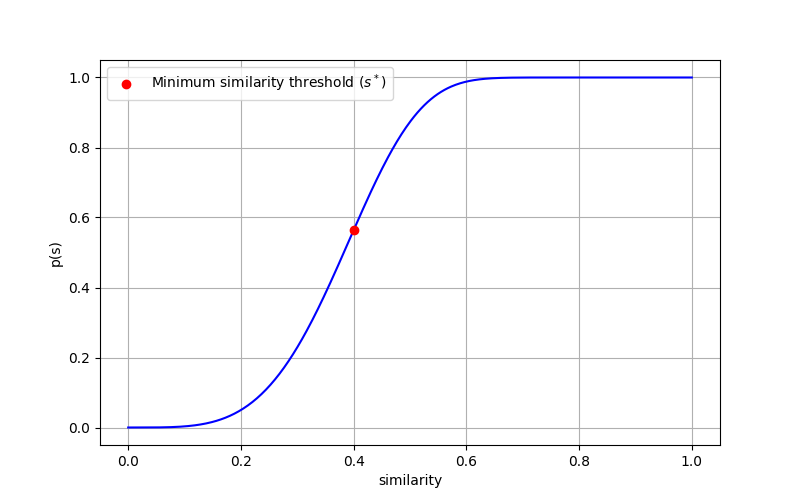
\includegraphics[width=0.8\textwidth]{Screenshot_1.png}
    \label{fig:placeholder}
\end{figure}
shows the graph for the function $p(s)$ with b=32 and r=4 as parameters. The red dot is approximately 0.4 and is the minimum similarity threshold.

At this point we have all the elements necessary to define a specific procedure to find similar reviews, using Jaccard similarity as a similarity metric and using MinHashing and LSH to reduce the computational complexity.
\begin{enumerate}
    \item Pick a value of k (in our case k = 5) and $\forall$ document construct a set of k-shingles.
    \item Pick a length n for the Min-Hash signatures (in our case n = 128), and construct the signature matrix having dimensions $n \times D$, where D is the number of reviews.
    \item Choose a threshold t (in our case t = 0.4) that defines how similar two documents have to be in order for them t be considered as "candidates" for the actual similarity computation. Then, pick the values of b (bands) and r (rows within a band) such that $br=n$ and $t \approx (\frac{1}{b})^\frac{1}{r}$ (in our case, b = 4 and r = 32).
    \item Construct the candidate pairs by applying LSH.
    \item Examine each candidate pair's signatures and determine whether the fraction of components in which they agree is at least t. 
\end{enumerate}
This is the procedure that has been implemented in the work done. In the next section the results obtained will be presented and commented on.

\section{Results}
At this point, having examined the techniques used in the project from both a theoretical perspective and the choice of parameters, some runs of the written code were performed and the results were combined. This is because subsampling is performed randomly, so different results can be obtained with each run.

These are the similar reviews obtained (remember, the minimum similarity threshold was set to 0.4). Only a few of the reviews are shown, as some are particularly long. The similar reviews are shown in ascending order of Jaccard similarity and, for each of them, there is a short comment that analizes the result obtained.

\begin{itemize}
    {\fontsize{9pt}{11pt}\selectfont
    \item Review 1: \textit{This book was in great condition and I received it in a timely manner. I was very pleased with the book.}
    \item Review 2: \textit{I received the book in good condition and in a timely manner}
    \item Jaccard similarity: 0.4219
    \item Considerations: we can see that some words are in common (such as "condition", "timely manner", "book"), so the reviews are quite similar.
    } 
\end{itemize}
\dotfill
\begin{itemize}
    {\fontsize{9pt}{11pt}\selectfont
    \item Review 1: \textit{I am very happy with this seller. The book arrived quickly as well as the condition it was described as.}
    \item Review 2: \textit{An imaginative novel by Mr. Archer. The book arrived in the condition described, and quickly after order.}
    \item Jaccard similarity: 0.4297
    \item Considerations: as in the previous result, some words are in common ("book", "condition", "quickly").
    }
\end{itemize}
\dotfill
\begin{itemize}
    {\fontsize{9pt}{11pt}\selectfont
    \item Review 1: \textit{Read this years ago and I wanted to read it again and have it for my library. Just as great as I remembered.}
    \item Review 2: \textit{I read it years ago and wanted to read it again before seeing the movie :) as great as I remember!}
    \item Jaccard similarity: 0.5078
    \item Considerations: here, some phrases are in common, such as "years ago", "wanted to read it again", "as great as I". 
    }
\end{itemize}
\dotfill
\begin{itemize}
    {\fontsize{9pt}{11pt}\selectfont
    \item Review 1: \textit{one of the best books she has written}
    \item Review 2: \textit{This was one of the best books I have ever read.}
    \item Jaccard similarity: 0.5469
    \item Considerations: "one of the best books" is in common for the two reviews, so we have a little bit stronger similarity than in the previous couple because it is a longer phrase. 
    }
\end{itemize}
\dotfill
\begin{itemize}
    {\fontsize{9pt}{11pt}\selectfont
    \item Review 1: \textit{My youngest daughter is an avid reader and loves re-reading books she was assigned in English class. In fact, she is a collector of these required assigned readings such as The Picture of Dorian Gray.}
    \item Review 2: \textit{My youngest daughter is an avid reader and loves re-reading books she was assigned in English class. In fact, she is a collector of these required assigned readings such as Of Mice and Men.}
    \item Jaccard similarity: 0.7578
    \item Considerations: almost identical reviews, but the first one ends with "The Picture of Dorian Gray" while the second one ends with "Of Mice and Men".
    }
\end{itemize}
\dotfill
\begin{itemize}
    {\fontsize{9pt}{11pt}\selectfont
    \item Review 1: \textit{.it was a freebie. it was a paperless book. why not take advantage of it right? not like WHOA! book!}
    \item Review 2: \textit{stocking up on freebies... .it was a freebie. it was a paperless book. why not take advantage of it right? not like WHOA! book!}
    \item Jaccard similarity: 0.8047
    \item Considerations: leaving aside the punctuation marks (which are obmitted in the normalization phase), the second review has a different start phrase but, after that, the two reviews are almost identical.
    }
\end{itemize}
\dotfill
\begin{itemize}
    {\fontsize{9pt}{11pt}\selectfont
    \item Review 1: \textit{Two teenagers from rival families fall in love, marry secretly, and take their own lives rather than live without each other. Despite the teenage melodrama, "Romeo and Juliet" remains one of Shakespeare's most enduring and popular plays, even if it wasn't his best -- lots of death, teen lovers and enchanting dialogue.In the city of Verona, the Montagues and Capulets are locked in a deadly feud. Then a Montague teen named Romeo, infatuated with a Capulet girl named Rosaline, sneaks into a party to see her.... but instead encounters another Capulet girl named Juliet, and the two immediately fall in love. Since their families hate each other, their love must be expressed in secret.Hoping to unite the two families, the kindly priest Friar Lawrence assists the two in marrying in secret. But then Juliet's cousin Tybalt challenges Romeo to a duel, leading to the death of two men -- and Romeo's exile from Verona. Even worse, the Capulets have decided to marry Juliet to Count Paris -- leading to a desperate plan that goes horribly awry.This edition also has Jacqueline Ritten's "Juliet's Story: A Retelling of Shakespeare's Romeo and Juliet," a rather nice if excessively "teenagerish" short story that tells of Juliet's memories and inner thoughts."Romeo and Juliet" is a play that is hard to pin down -- some see it as the poetry-laden embodiment of romantic love, while others view it as Shakespeare's witty jabs at fickle teenage infatuation and how melodramatic the kids are (Juliet is only thirteen!). But whatever you think it is, it's undeniable that it's a beautifully written, often-wrenching story.Despite the simplicity of the story, Shakespeare spins it in a silken web of lush poetry ("O swear not by the moon, the inconstant moon/That monthly changes in her circled orb") and the famous speeches where Romeo and Juliet speak at night on a balcony. The mostly romantic play takes a dark turn towards the end, when only a few minutes might have changed the fates of "Juliet and her Romeo."And Shakespeare seems rather fond of his characters here, depicting Romeo as a passionate young boy and Juliet as rather sweetly insecure young girl; there's also a fairly good cast of young men whose spirits are more elevated than their brains, and the kindly friar who rather naively hopes to use the kids to create peace.But Shakespeare was also clearly aware that passionate teenage love is not necessarily the truest love ("Young men's love then lies/Not truly in their hearts, but in their eyes"), and leaves you wondering what might have happened if Romeo and Juliet had lived.Whether a gentle mockery of young love or a passionate, idealized romance, "Romeo and Juliet" is a timeless and lovely little play. Not the best of the Bard, but still quite good.}
    \item Review 2: \textit{Two teenagers from rival families fall in love, marry secretly, and take their own lives rather than live without each other. Despite the teenage melodrama, "Romeo and Juliet" remains one of Shakespeare's most enduring and popular plays, even if it wasn't his best -- lots of death, teen lovers and enchanting dialogue.In the city of Verona, the Montagues and Capulets are locked in a deadly feud. Then a Montague teen named Romeo, infatuated with a Capulet girl named Rosaline, sneaks into a party to see her.... but instead encounters another Capulet girl named Juliet, and the two immediately fall in love. Since their families hate each other, their love must be expressed in secret.Hoping to unite the two families, the kindly priest Friar Lawrence assists the two in marrying in secret. But then Juliet's cousin Tybalt challenges Romeo to a duel, leading to the death of two men -- and Romeo's exile from Verona. Even worse, the Capulets have decided to marry Juliet to Count Paris -- leading to a desperate plan that goes horribly awry."Romeo and Juliet" is a play that is hard to pin down -- some see it as the poetry-laden embodiment of romantic love, while others view it as Shakespeare's witty jabs at fickle teenage infatuation and how melodramatic the kids are (Juliet is only thirteen!). But whatever you think it is, it's undeniable that it's a beautifully written, often-wrenching story.Despite the simplicity of the story, Shakespeare spins it in a silken web of lush poetry ("O swear not by the moon, the inconstant moon/That monthly changes in her circled orb") and the famous speeches where Romeo and Juliet speak at night on a balcony. The mostly romantic play takes a dark turn towards the end, when only a few minutes might have changed the fates of "Juliet and her Romeo."And Shakespeare seems rather fond of his characters here, depicting Romeo as a passionate young boy and Juliet as rather sweetly insecure young girl; there's also a fairly good cast of young men whose spirits are more elevated than their brains, and the kindly friar who rather naively hopes to use the kids to create peace.But Shakespeare was also clearly aware that passionate teenage love is not necessarily the truest love ("Young men's love then lies/Not truly in their hearts, but in their eyes"), and leaves you wondering what might have happened if Romeo and Juliet had lived.The annotated edition is a very good one, especially for people who are just starting out on Shakespeare -- a couple of well-written, respectful introductions and extensive annotation that is useful but not intrusive. Whenever there's a word that is unclear in meaning or different from how it was once perceived, there's a little tip at the bottom of the page.Whether a gentle mockery of young love or a passionate, idealized romance, "Romeo and Juliet" is a timeless and lovely little play. Not the best of the Bard, but still quite good.}
    \item Jaccard similarity: 0.8516
    \item Considerations: two very long reviews which are almost identical, but the first one contains this phrase: \textit{"This edition also has Jacqueline Ritten's "Juliet's Story: A Retelling of Shakespeare's Romeo and Juliet," a rather nice if excessively "teenagerish" short story that tells of Juliet's memories and inner thoughts."}, while the second one contains this phrase: \textit{"The annotated edition is a very good one, especially for people who are just starting out on Shakespeare -- a couple of well-written, respectful introductions and extensive annotation that is useful but not intrusive. Whenever there's a word that is unclear in meaning or different from how it was once perceived, there's a little tip at the bottom of the page."} These two differences makes the similarity between the two reviews to decrease because of its lenght, even if it remains quite high since most of the text remains identical.
    }
\end{itemize}
\dotfill
\begin{itemize}
    {\fontsize{9pt}{11pt}\selectfont
    \item Review 1: \textit{I don't recommend you this abridged audio book. Please get the complete audio, and that's why.This book is so widely cited and interpreted contrary to the author's original thought, that every economist should read it completely to avoid being misled by such incorrect interpretations.First, let us take the "invisible hand" metaphor. When I have studied economy in the University, I was taught that almost the entire book is devoted to the "invisible hand" which means "self-corrective markets", "liberalism", "Laissez-faire" and "state non-intervention". After reading this book, I have found out that Adam Smith did use the term "invisible hand" only once in the entire book, in the discussion of domestic versus foreign trade.To illustrate the point, let me quote the text where term "invisible hand" is used: "First, every individual endeavours to employ his capital as near home as he can, and consequently as much as he can in the support of domestic industry, provided always that he can thereby obtain the ordinary, or not a great deal less than the ordinary profits of stock. Thus, upon equal, or nearly equal profits, every wholesale merchant naturally prefers the home trade to the foreign trade of consumption, and the foreign trade of consumption to the carrying trade. In the home trade, his capital is never so long out of his sight as it frequently is in the foreign trade of consumption. [...]Secondly, every individual who employs his capital in the support of domestic industry, necessarily endeavours so to direct that industry, that its produce may be of the greatest possible value. [...]As every individual, therefore, endeavours as much as he can, both to employ his capital in the support of domestic industry, and so to direct that industry that its produce maybe of the greatest value; every individual necessarily labours to render the annual revenue of the society as great as he can. He generally, indeed, neither intends to promote the public interest, nor knows how much he is promoting it. By preferring the support of domestic to that of foreign industry, he intends only his own security; and by directing that industry in such a manner as its produce may be of the greatest value, he intends only his own gain; and he is in this, as in many other cases, led by an invisible hand to promote an end which was no part of his intention. Nor is it always the worse for the society that it was no part of it."After reading this book, I have found out that Adam Smith was influenced by French Physiocrats. The Physiocrats saw the true wealth of a nation as determined by the surplus of agricultural production over and above that needed to support agriculture (by feeding farm labourers and so forth). Other forms of economic activity, such as manufacturing, were viewed as taking this surplus agricultural production and transforming it into new products, by using the surplus agricultural production to feed the workers who produced the extra goods. While these manufacturers and other non agricultural workers may be useful, they were seen as 'sterile' in that their income derives ultimately not from their own work, but from the surplus production of the agricultural sector.I have found out that this book is not about "invisible hand" or "Laissez-faire". It is quite a complete study that covers almost every basic aspect of the economy, and remains an effective introduction to economics to this day.This book is so often mischaracterized and politicized that I suggest you to listen it completely by yourself. This is a must read for every economist. You can get the complete unabridged audio version of this book.}
    \item Review 2: \textit{This book is so widely cited and interpreted contrary to the author's original thought, that every economist should read it completely to avoid being misled by such incorrect interpretations.First, let us take the "invisible hand" metaphor. When I have studied economy in the University, I was taught that almost the entire book is devoted to the "invisible hand" which means "self-corrective markets", "liberalism", "Laissez-faire" and "state non-intervention". After reading this book, I have found out that Adam Smith did use the term "invisible hand" only once in the entire book, in the discussion of domestic versus foreign trade.To illustrate the point, let me quote the text where term "invisible hand" is used: "First, every individual endeavours to employ his capital as near home as he can, and consequently as much as he can in the support of domestic industry, provided always that he can thereby obtain the ordinary, or not a great deal less than the ordinary profits of stock. Thus, upon equal, or nearly equal profits, every wholesale merchant naturally prefers the home trade to the foreign trade of consumption, and the foreign trade of consumption to the carrying trade. In the home trade, his capital is never so long out of his sight as it frequently is in the foreign trade of consumption. [...]Secondly, every individual who employs his capital in the support of domestic industry, necessarily endeavours so to direct that industry, that its produce may be of the greatest possible value. [...]As every individual, therefore, endeavours as much as he can, both to employ his capital in the support of domestic industry, and so to direct that industry that its produce maybe of the greatest value; every individual necessarily labours to render the annual revenue of the society as great as he can. He generally, indeed, neither intends to promote the public interest, nor knows how much he is promoting it. By preferring the support of domestic to that of foreign industry, he intends only his own security; and by directing that industry in such a manner as its produce may be of the greatest value, he intends only his own gain; and he is in this, as in many other cases, led by an invisible hand to promote an end which was no part of his intention. Nor is it always the worse for the society that it was no part of it."After reading this book, I have found out that Adam Smith was influenced by French Physiocrats. The Physiocrats saw the true wealth of a nation as determined by the surplus of agricultural production over and above that needed to support agriculture (by feeding farm labourers and so forth). Other forms of economic activity, such as manufacturing, were viewed as taking this surplus agricultural production and transforming it into new products, by using the surplus agricultural production to feed the workers who produced the extra goods. While these manufacturers and other non agricultural workers may be useful, they were seen as 'sterile' in that their income derives ultimately not from their own work, but from the surplus production of the agricultural sector.I have found out that this book is not about "invisible hand" or "Laissez-faire". It is quite a complete study that covers almost every basic aspect of the economy, and remains an effective introduction to economics to this day. Just don't start reading economic books from this book. It would be hard to understand. It assumes that you already have economics background, i.e. have studied economics for a few years.This book is so often mischaracterized and politicized that I suggest you to read it completely by yourself. This is a must read for every economist. You can get an audio version of this book to avoid lengthy read.}
    \item Jaccard similarity: 0.9062
    \item Considerations: similarly as the previous couple, the first one contains this phrase: \textit{"I don't recommend you this abridged audio book. Please get the complete audio, and that's why."} while the second one contains this phrase: \textit{"Just don't start reading economic books from this book. It would be hard to understand. It assumes that you already have economics background, i.e. have studied economics for a few years."}. Being two shorter phrases than before, the similarity is higher.
    }
\end{itemize}
\begin{itemize}
    {\fontsize{9pt}{11pt}\selectfont
    \item Review 1: \textit{Basil, who up until now was a mediocre painter after meeting Dorian Gray a young Adonis, was inspired to create a masterpiece of which he puts himself into. Against Basil's wishes, Dorian Gray is influenced by Basil's friend Lord Henry. Dorian looks at his portrait and realizes that while the portrait will stay young forever, he will grow old; so Dorian makes a wish that if only he could stay young forever and the portrait can age.At first Dorian does not realize his wishes been granted. He falls in love with a beautiful young actress who is every woman that Shakespeare ever wrote about. But once again due to Lord Henry's influence, he realizes that she's just a common girl.Starting with absent-minded acts Dorian slowly sinks into debauchery. And with every new act his picture becomes more grotesque while Dorian stays is young and as innocent looking as the day his picture was painted.What will become of Dorian?What will become of Dorian's painting?What would you do if you were Dorian?Oscar Wilde paints a picture himself as he describes Dorian Gray's dilemma. And we as readers travel with Dorian as each decision is made. In some places in the story Oscar Wilde seems to drag on and on with detail; however we find that this detail is necessary to set the next scene.Oscar Wilde himself led a risky life that lead to a jail sentence; is attitudes can be seen in the dialogues in this book.}
    \item Review 2: \textit{Basil, who up until now was a mediocre painter after meeting Dorian Gray a young Adonis, was inspired to create a masterpiece of which he puts himself into. Against Basil's wishes, Dorian Gray is influenced by Basil's friend Lord Henry. Dorian looks at his portrait and realizes that while the portrait will stay young forever, he will grow old; so Dorian makes a wish that if only he could stay young forever and the portrait can age.At first Dorian does not realize his wishes been granted. He falls in love with a beautiful young actress who is every woman that Shakespeare ever wrote about. But once again due to Lord Henry's influence, he realizes that she's just a common girl.Starting with absent-minded acts Dorian slowly sinks into debauchery. And with every new act his picture becomes more grotesque while Dorian stays is young and as innocent looking as the day his picture was painted.What will become of Dorian?What will become of Dorian's painting?What would you do if you were Dorian?Oscar Wilde paints a picture himself as he describes Dorian Gray's dilemma. And we as readers travel with Dorian as each decision is made. In some places in the story Oscar Wilde seems to drag on and on with detail; however we find that this detail is necessary to set the next scene.Oscar Wilde himself led a risky life that lead to a jail sentence; is attitudes can be seen in the dialogues in this book.The Picture of Dorian Gray Starring: George Sanders, Hurd Hatfield}
    \item Jaccard similarity: 0.9219
    \item Considerations: here, the only difference is that the second review contains this phrase: \textit{"The Picture of Dorian Gray Starring: George Sanders, Hurd Hatfield"}. The rest of the text is identical.
    }
\end{itemize}
\dotfill
\begin{itemize}
    {\fontsize{9pt}{11pt}\selectfont
    \item Review 1: \textit{Wuthering Heights has been reviewed ad infinitum, but I wanted to say that this is one of the most beautiful books I own.I was looking for a series of classics that I could purchase in hardcover to spruce up my personal library. I stumbled upon these special editions from Penguin Classics, with covers designed by Coralie Bickford-Smith. I love books, but these books still make me giddy with delight when I pick them up. The covers have so much character and they're sturdy. The fonts are classic and easy to read, and the paper is substantial. The ribbon bookmarks, that match the cover, are a really nice touch. The only bad thing I can say, and it's so minor, is that the binding is a little stiff when the book is new. It loosens as you read.There are more titles available, though some are still exclusive to the UK. I truly hope Amazon and Penguin make all editions available in the US and keep them coming!}
    \item Review 2: \textit{Sense \& Sensibility has been reviewed ad infinitum, but I wanted to say that this is one of the most beautiful books I own.I was looking for a series of classics that I could purchase in hardcover to spruce up my personal library. I stumbled upon these special editions from Penguin Classics, with covers designed by Coralie Bickford-Smith. I love books, but these books still make me giddy with delight when I pick them up. The covers have so much character and they're sturdy. The fonts are classic and easy to read, and the paper is substantial. The ribbon bookmarks, that match the cover, are a really nice touch. The only bad thing I can say, and it's so minor, is that the binding is a little stiff when the book is new. It loosens as you read.There are more titles available, though some are still exclusive to the UK. I truly hope Amazon and Penguin make all editions available in the US and keep them coming!}
    \item Jaccard similarity: 0.9375
    \item Considerations: here, the only difference is that the first review starts with \textit{"Wuthering Heights"} while the second one starts with \textit{"Sense \& Sensibility"}.
    }
\end{itemize}
\dotfill
\begin{itemize}
    {\fontsize{9pt}{11pt}\selectfont
    \item Review 1: \textit{I realized what Amazon does.-- They pool audio and text reviews and place all of those reviews on each of the products' pages, regardless of form the material is taking. You wouldn't expect a book review on the DVD's page. In this case, every word is the same, but a book review tells you only about the story, not the quality of the audio product.-- But any regular audiobook listener has experienced a great book poorly read, or hammed up, or a voice that grated on your nerves, or found a book you loved to listen to, but couldn't find the time to sit and read (Lord of the Rings for me).-- A review of the author's work tells you NOTHING about the audio, and yet, if you try and find what you're getting into, you have to sift through MANY book reviews before finding out the quality of the voice work, as most people have reviewed the author and the book, rather than the audiobook.-- So, here's a small review of the audiobook, if you're interested in purchasing that. If you're looking for a review of the author, I am not being unhelpful, but Amazon is. I will request that they change their policy and display the reviews separately.... Jim Dale is one of the best voice actors I've ever listened to and he brought the books to life an a way that reading could never do. I like reading, but it's really incredible to have someone put a different voice to every character, displaying the emotions and tone of the interactions.... They are a really phenomenal experience, and I've listened to them over again and again.}
    \item Review 2: \textit{EDIT: Some people mark audio reviews as "unhelpful", which I found strange, until I realized what Amazon does.-- They pool audio and text reviews and place all of those reviews on each of the products' pages, regardless of form the material is taking. You wouldn't expect a book review on the DVD's page. In this case, every word is the same, but a book review tells you only about the story, not the quality of the audio product.-- But any regular audiobook listener has experienced a great book poorly read, or hammed up, or a voice that grated on your nerves, or found a book you loved to listen to, but couldn't find the time to sit and read (Lord of the Rings for me).-- A review of the author's work tells you NOTHING about the audio, and yet, if you try and find what you're getting into, you have to sift through MANY book reviews before finding out the quality of the voice work, as most people have reviewed the author and the book, rather than the audiobook.-- So, here's a small review of the audiobook, if you're interested in purchasing that. If you're looking for a review of the author, I am not being unhelpful, but Amazon is. I will request that they change their policy and display the reviews separately.... Jim Dale is one of the best voice actors I've ever listened to and he brought the books to life an a way that reading could never do. I liked reading the books, but it's really incredible to have someone put a different voice to every character, displaying the emotions and tone of the interactions.... They are a really phenomenal experience, and I've listened to them over again and again.}
    \item Jaccard similarity: 0.9766
    }
\end{itemize}
\dotfill
\begin{itemize}
    {\fontsize{9pt}{11pt}\selectfont
    \item Review 1: \textit{I love the New King James Version, put out by Thomas Nelson, but I loath Thomas Nelson Bibles. This is how I happened upon the Thompson a few years ago as I was relieved to find a NKJV not made by T.N. I first bought an NKJV in bonded leather. After 2 years of very heavy use, I bought an NKJV in genuine leather, and later a handy size KJV in genuine. All three of these Bibles are wonderful in every way.The Thompson Study system is very helpful and they've graciously spared us from a myriad of religious cliche and personal opinion. The page layout is smart. The Bible text actually fills the page and all study helps and references are relegated to the side margins. There are so many ways to use the studies and references, I am unable to number them here. The concordance is as extensive as any I've seen. The 14 maps are colorful and very well done. Simply put, it's a complete, Jesus-exalting study Bible designed with excellence.The construction of these Bibles is equally impressive. The paper is just right--not too thick, not too thin. The print is dark and sharp. Their font is subtil and very appropriate for the Bible, if you ask me. The red words of Jesus are RED. They're not muddy brown; they're not pink; they're bright, deep, beautiful red. They are printed consistantly page to page, not some pages lighter or misprinted, as the Thomas Nelson folks are plagued by.Now that I own three Thompsons, I feel about them the way a good ol' boy down in the South feels about shotguns. \&quot;I have more than I need, but not as many as I want!\&quot;}
    \item Review 2: \textit{I love the New King James Version, put out by Thomas Nelson, but I loath Thomas Nelson Bibles. This is how I happened upon the Thompson a few years ago as I was relieved to find a NKJV not made by T.N. I first bought an NKJV in bonded leather. After 2 years of very heavy use, I bought an NKJV in genuine leather, and later a handy size KJV in genuine. All three of these Bibles are wonderful in every way.The Thompson Study system is very helpful and they've graciously spared us from a myriad of religious cliche and personal opinion. The page layout is smart. The Bible text actually fills the page and all study helps and references are relegated to the side margins. There are so many ways to use the studies and references, I am unable to number them here. The concordance is as extensive as any I've seen. The 14 maps are colorful and very well done. Simply put, it's a complete, Jesus-exalting study Bible designed with excellence.The construction of these Bibles is equally impressive. The paper is just right--not too thick, not too thin. The print is dark and sharp. Their font is subtil and very appropriate for the Bible, if you ask me. The red words of Jesus are RED. They're not muddy brown; they're bright, deep, beautiful red. They are printed consistantly page to page, not some pages lighter or misprinted, as the Thomas Nelson folks are plagued by.Now that I own three Thompsons, I feel about them the way a good ol' boy down in the South feels about shotguns. \&quot;I have more than I need, but not as many as I want!\&quot;}
    \item Jaccard similarity: 0.9922
    \item Considerations: almost identical reviews as the similarity very close to 1 shows. The only difference is that the second review contains this phrase: \textit{"not pink; they're "}.
    }
\end{itemize}
\dotfill 

It can be noted that longer reviews showed higher Jaccard similarity values. This is likely due to the fact that, with longer texts available, more shingles are generated and therefore, even in the presence of text differences, there will be many more identical shingles than different ones. On the other hand, similar text differences in shorter texts have a greater impact due to the reduced number of shingles generated, except for review pairs close to the minimum similarity threshold, for which the similarity is due to the presence of common words and short phrases.

\vspace{6cm}

\textit{I declare that this material, which I now submit for assessment, is entirely my own work and has not been taken from the work of others, save and to the extent that such work has been cited and acknowledged within the text of my work. I understand that plagiarism, collusion, and copying are grave and serious offences in the university and accept the penalties that would be imposed should I engage in plagiarism, collusion or copying. This assignment, or any part of it, has not been previously submitted by me or any other person for assessment on this or any other course of study. No generative AI tool has been used to write the code or the report content.}

\vspace{6cm}
\printbibliography
\end{document}


